% Template for Elsevier CRC journal article
% version 1.2 dated 08 January 2015

% This file (c) 2009-15 Elsevier Ltd.  Modifications may be freely made,
% provided the edited file is saved under a different name

% This file contains modifications for Nuclear and Particle Physics Proceedings

% Changes since version 1.0
% - elsarticle class option changed from 1p to 3p (to better reflect CRC layout)
%
% version 1.2
% - Journal name changed to "Nuclear and Particle Physics Proceedings"

%-----------------------------------------------------------------------------------

%% This template uses the elsarticle.cls document class and the extension package ecrc.sty
%% For full documentation on usage of elsarticle.cls, consult the documentation "elsdoc.pdf"
%% Further resources available at http://www.elsevier.com/latex

%-----------------------------------------------------------------------------------

%%%%%%%%%%%%%%%%%%%%%%%%%%%%%%%%%%%%%%%%%%%%%%
%%%%%%%%%%%%%%%%%%%%%%%%%%%%%%%%%%%%%%%%%%%%%%
%%                                          %%
%% Important note on usage                  %%
%% -----------------------                  %%
%% This file must be compiled with PDFLaTeX %%
%% Using standard LaTeX will not work!      %%
%%                                          %%
%%%%%%%%%%%%%%%%%%%%%%%%%%%%%%%%%%%%%%%%%%%%%%
%%%%%%%%%%%%%%%%%%%%%%%%%%%%%%%%%%%%%%%%%%%%%%

%-------NEW COMMANDS------------
\newcommand{\trento}{T\raisebox{-0.5ex}{R}ENTo}

%-------pic folder--------------



%% The '3p' and 'times' class options of elsarticle are used for Elsevier CRC
\documentclass[3p,times,twocolumn]{elsarticle}

%% The `ecrc' package must be called to make the CRC functionality available
\usepackage{ecrc}
\graphicspath{{fig/}}
\usepackage{tabularx}
%% The ecrc package defines commands needed for running heads and logos.
%% For running heads, you can set the journal name, the volume, the starting page and the authors

%% set the volume if you know. Otherwise `00'
\volume{00}

%% set the starting page if not 1
\firstpage{1}

%% Give the name of the journal
\journalname{Nuclear and Particle Physics Proceedings}

%% Give the author list to appear in the running head
%% Example \runauth{C.V. Radhakrishnan et al.}
\runauth{}

%% The choice of journal logo is determined by the \jid and \jnltitlelogo commands.
%% A user-supplied logo with the name <\jid>logo.pdf will be inserted if present.
%% e.g. if \jid{yspmi} the system will look for a file yspmilogo.pdf
%% Otherwise the content of \jnltitlelogo will be set between horizontal lines as a default logo

%% Give the abbreviation of the Journal.
\jid{nppp}

%% Give a short journal name for the dummy logo (if needed)
\jnltitlelogo{Nuclear and Particle Physics Proceedings}

%% Hereafter the template follows `elsarticle'.
%% For more details see the existing template files elsarticle-template-harv.tex and elsarticle-template-num.tex.

%% Elsevier CRC generally uses a numbered reference style
%% For this, the conventions of elsarticle-template-num.tex should be followed (included below)
%% If using BibTeX, use the style file elsarticle-num.bst

%% End of ecrc-specific commands
%%%%%%%%%%%%%%%%%%%%%%%%%%%%%%%%%%%%%%%%%%%%%%%%%%%%%%%%%%%%%%%%%%%%%%%%%%

%% The amssymb package provides various useful mathematical symbols
\usepackage{amssymb}
%% The amsthm package provides extended theorem environments
%% \usepackage{amsthm}

%% The lineno packages adds line numbers. Start line numbering with
%% \begin{linenumbers}, end it with \end{linenumbers}. Or switch it on
%% for the whole article with \linenumbers after \end{frontmatter}.
%% \usepackage{lineno}

%% natbib.sty is loaded by default. However, natbib options can be
%% provided with \biboptions{...} command. Following options are
%% valid:

%%   round  -  round parentheses are used (default)
%%   square -  square brackets are used   [option]
%%   curly  -  curly braces are used      {option}
%%   angle  -  angle brackets are used    <option>
%%   semicolon  -  multiple citations separated by semi-colon
%%   colon  - same as semicolon, an earlier confusion
%%   comma  -  separated by comma
%%   numbers-  selects numerical citations
%%   super  -  numerical citations as superscripts
%%   sort   -  sorts multiple citations according to order in ref. list
%%   sort&compress   -  like sort, but also compresses numerical citations
%%   compress - compresses without sorting
%%
%% \biboptions{comma,round}

% \biboptions{}

% if you have landscape tables
\usepackage[figuresright]{rotating}

% put your own definitions here:
%   \newcommand{\cZ}{\cal{Z}}
%   \newtheorem{def}{Definition}[section]
%   ...

% add words to TeX's hyphenation exception list
%\hyphenation{author another created financial paper re-commend-ed Post-Script}

% declarations for front matter

\begin{document}

\begin{frontmatter}

%% Title, authors and addresses

%% use the tnoteref command within \title for footnotes;
%% use the tnotetext command for the associated footnote;
%% use the fnref command within \author or \address for footnotes;
%% use the fntext command for the associated footnote;
%% use the corref command within \author for corresponding author footnotes;
%% use the cortext command for the associated footnote;
%% use the ead command for the email address,
%% and the form \ead[url] for the home page:
%%
%% \title{Title\tnoteref{label1}}
%% \tnotetext[label1]{}
%% \author{Name\corref{cor1}\fnref{label2}}
%% \ead{email address}
%% \ead[url]{home page}
%% \fntext[label2]{}
%% \cortext[cor1]{}
%% \address{Address\fnref{label3}}
%% \fntext[label3]{}

\dochead{}
%% Use \dochead if there is an article header, e.g. \dochead{Short communication}

\title{Constaints on rapidity-dependent initial conditions from particle charged particle pseudorapidity densities and correlations at LHC}

%% use optional labels to link authors explicitly to addresses:
%% \author[label1,label2]{<author name>}
%% \address[label1]{<address>}
%% \address[label2]{<address>}

\author{Weiyao Ke}
\author{J. Scott Moreland}
\author{Jonah E. Bernhard}
\author{Steffen A. Bass}

\address{Department of Physics, Duke University, Durham, NC 27708-0305, United States}

\begin{abstract}
The initial three-dimensional entropy distribution of the quark-gluon plasma produced in relativistic heavy-ion collision is contained using LHC charged particle data.
We use a cumulant generating function approach to parametrize the rapidity dependence of local entropy deposition and extend mid-rapidity initial condition model \trento~to finite rapidity.
The initial condition model is compared to centrality dependent charged particle pseudorapidity densities
of p+Pb (5.02A TeV) and Pb+Pb (2.76A TeV) and parameters are optimized using Bayesian technique.
Different parametrizations are then selected by comparing to two-particle psuedorapidity correlations.
Using the selected parametrization and optimized parameters, we calculated rapidity dependent flows, event-plane decorrelations.

\end{abstract}

\begin{keyword}
initial condition \sep charged particle density \sep two-particle correlation
%% keywords here, in the form: keyword \sep keyword

%% MSC codes here, in the form: \MSC code \sep code
%% or \MSC[2008] code \sep code (2000 is the default)

\end{keyword}

\end{frontmatter}

%%
%% Start line numbering here if you want
%%
% \linenumbers

%% main text
\section{Introduction}
\label{Introduction}
Ultra-relativistic heavy-ion collisions produce a strongly coupled quark-gluon plasma (sQGP) whose dynamics is well described by hydrodynamic-based models.
A small specific shear viscosity ($\eta/s$) is found to explain the experimental observations in previous studies.
A prerequisite and also a major source of uncertainty in hydrodynamic simulations is an initial condition which specifies the spatial entropy / energy distribution at some early time of the collision.
Most current initial condition models are longitudinal independent, which assume boost-invariance of the collision dynamics.
However, this assumption is explicitly broken in small collision systems such as p+Pb.
Even in central Pb+Pb collision, nucleon position fluctuations could introduce intricate local longitudinal dependence, which may affect the calculation of longitudinal dependent observables and hard-soft correlations.

Previous works approach the three-dimensional initial conditions using different physical pictures, from MC Glauber extensions, microscopic hadron transport, minijet productions and string formations to most recent developments in CGC effective field theory.
In this work, we use a parametric initial condition which encodes different types of longitudinal entropy deposition schemes with tunable parameters.
Although compared to previous models it does not reveal the physical mechanisms behind, the true value of a parametric model is that it tells what the initial condition might look like after performing a model-to-data comparison to optimize its parameters.
In fact, it is also a non-trivial task to infer the local longitudinal dependence of the initial fireball from final state observables.
The optimized model can then be fed into the state-of-the-art hydrodynamic and hybrid simulation to study the effect of longitudinal dynamics and fluctuations on annisotropic flows, event-plane decorrelations and other observables.

\section{Initial Condition Model}
\label{Model}
We extend the boost-invariant parametric initial condition model \trento~to include local longitudinal dependence by a cumulant generating function approach.
The physics of \trento~is described in reference \cite{Moreland:2014oya}. 
Using Bayesian techniques, it has been shown that the calibrated \trento~initial condition together with 2+1D viscous hydrodynamics Vishnew and UrQMD hadron rescattering afterburner can explain annisotropic flows, particle yields and mean transverse momentum at mid-rapidity to unprecedent level of accuracy.

The three dimensional extension proceed as following. 
Assuming the longitudinal asymmetry of local entropy deposition is triggered by the imbalance between incoming nuclear thickness function $T_A(\vec{x}_{\perp})$ and $T_B(\vec{x}_{\perp})$, we therefore parametrize the fist three rapidity-cumulant of the local entropy distribution function in terms of nuclear $T_A(\vec{x}_{\perp})$ and $T_B(\vec{x}_{\perp})$,
\begin{eqnarray}
\frac{ds(\vec{x}_{\perp}, \eta_s)}{dx_{\perp}^2 dy} \propto f(\vec{x}_{\perp})g(y; \mu(\vec{x}_{\perp}), \sigma(\vec{x}_{\perp}), \gamma(\vec{x}_{\perp}))\frac{dy}{d\eta}.
\end{eqnarray}
Here, $f(\vec{x}_{\perp})$ is the entropy calculated from boost-invariant \trento~model. Function $g(y; \mu, \sigma, \gamma)$ encodes the longitudinal dependence with its mean ($\mu$), standard deviation ($\sigma$) and skewness ($\gamma$) parametrized from $T_A$ and $T_B$.
We tests two parametrization as shown in table \ref{tab:parametrization}

\begin{table}
  \caption{
    \label{tab:parametrization}
    Rapidity-dependent initial condition parametrizations with two different models for the skewness parameter. The constant $T_0 = 1$~fm$^{-2}$ preserves desired dimensionality.
  }
  \begin{tabular}{cccc}
\hline\hline
      & \multicolumn{3}{c}{Distribution cumulant:} \\
      Model & \multicolumn{1}{c}{mean $\mu$} & \multicolumn{1}{c}{std.\ $\sigma$} & \multicolumn{1}{c}{skewness $\gamma$} \\
\hline
        Relative  & $\frac{1}{2} \mu_0 \log(T_A/T_B)$ & $\sigma_0$ & $\gamma_0 \frac{T_A - T_B}{T_A + T_B}$ \smallskip \\
        Absolute & $\frac{1}{2} \mu_0 \log(T_A/T_B)$  & $\sigma_0$ & $\gamma_0 (T_A - T_B)/T_0$ \\
\hline\hline
  \end{tabular}
\end{table}

\begin{figure}
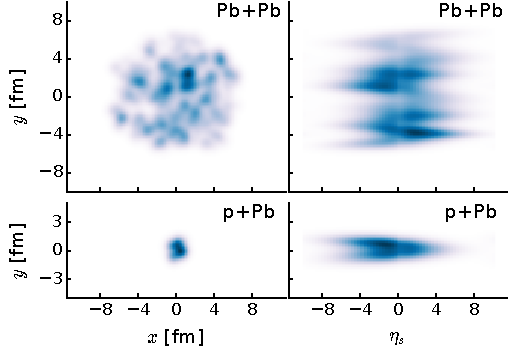
\includegraphics[width=\columnwidth]{trento3d_example.pdf}
\end{figure}

\section{Result}
\begin{figure*}
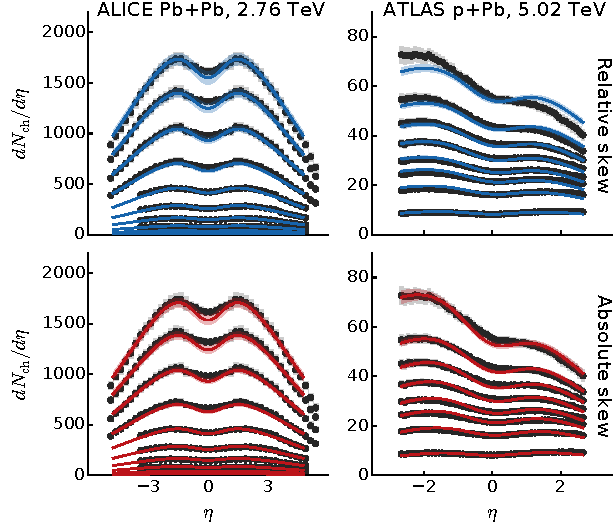
\includegraphics{chg_particle_rapidity.pdf}
\hfill
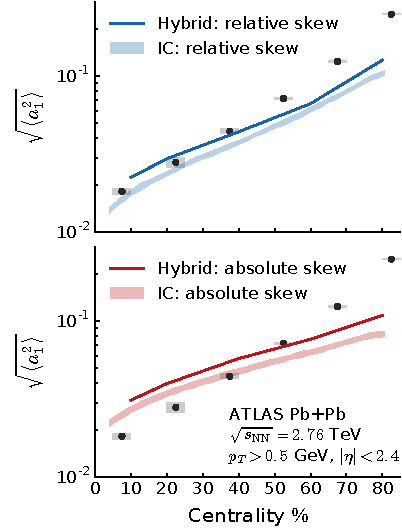
\includegraphics{fw_correlation_a1.pdf}
\end{figure*}

\begin{figure*}
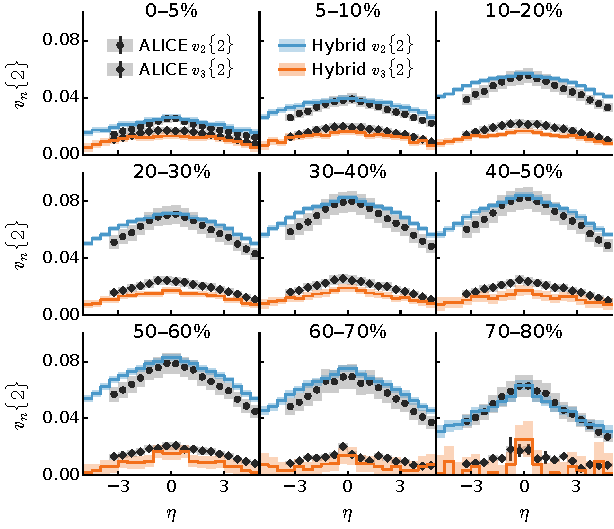
\includegraphics{vn_eta.pdf}
\hfill
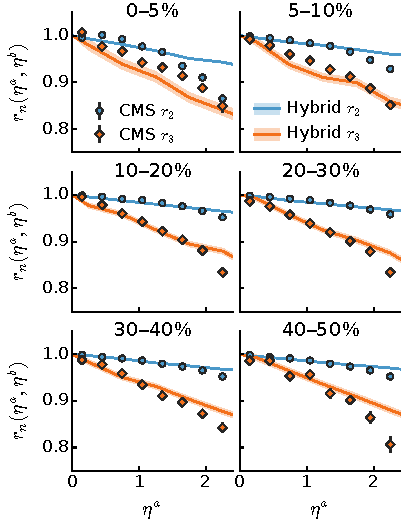
\includegraphics{evt_pln_decorr.pdf}
\end{figure*}
\label{Result}

\section{Conclusion}
\label{Conclusion}

%% The Appendices part is started with the command \appendix;
%% appendix sections are then done as normal sections
%% \appendix

%% \section{}
%% \label{}

%% References
%%
%% Following citation commands can be used in the body text:
%% Usage of \cite is as follows:
%%   \cite{key}         ==>>  [#]
%%   \cite[chap. 2]{key} ==>> [#, chap. 2]
%%

%% References with BibTeX database:
%%\nocite{*}
\bibliographystyle{elsarticle-num}
\bibliography{trento3d}

%% Authors are advised to use a BibTeX database file for their reference list.
%% The provided style file elsarticle-num.bst formats references in the required Procedia style

%% For references without a BibTeX database:

% \begin{thebibliography}{00}

%% \bibitem must have the following form:
%%   \bibitem{key}...
%%

% \bibitem{}

% \end{thebibliography}

\end{document}

%%
%% End of file `nuphbp-template.tex'. 
